\chapter{An Introduction to the GSAS-II GUI}
\label{Chap:GSASIIintro}

 I will provide an overview to how GSAS-II is organized now because in subsequent chapters of this book, I will frequently alternate between introducing concepts and then showing how those concepts are embodied within GSAS-II. I think that having a familiarity with the organization of GSAS-II will be helpful before this. For this reason I want to provide an orientation for how GSAS-II is installed and organized here.

\section{Installing GSAS-II \& Web Resources}
GSAS-II is hosted on GitHub.com and is typically downloaded from there. Links to information provided about GSAS-II is provided on the GitHub home page, \texttt{https://GSASII.github.io}.\index{GSAS-II home page} For installation instructions\index{GSAS-II installation instructions}, please see the installation section of that website (\texttt{https://advancedphotonsource.github.io/GSAS-II-tutorials/install.html}) . Most people will choose to download one of the GSAS2MAIN self-installers, but there are many different ways that GSAS-II can be installed depending on your own preferences and goals. The installation instructions web pages provide a detailed  discussion of the options and advantages. 

The source code for GSAS-II is found in GitHub repository  \texttt{https://github.com/AdvancedPhotonSource/GSAS-II}. It is worth noting that the source code for GSAS-II is installed as part of the GSAS-II installation, so we try to keep the size of that repo small. Thus, there are three other repositories associated with GSAS-II with material that is less frequently downloaded. The GSAS-II documentation, including tutorial web pages, and input used to create  the web pages, help pages and newer tutorials is found at \texttt{https://github.com/AdvancedPhotonSource/GSAS-II-tutorials}. Routines used to compile and package GSAS-II, as well as the distribution files for installation are found in repo https://github.com/AdvancedPhotonSource/GSAS-II-buildtools and finally the files used to create this book are found at \texttt{https://github.com/briantoby/PowderCrystallography}. There is also a GSAS-II code developer's manual, which is a formatted version of text and comments found in the source code. This is hosted on a separate site, \texttt{https://gsas-ii.readthedocs.io/}.\index{GSAS-II Developer's manual} The documentation section of the GSAS-II home page provides access to the manuals in several formats. 

\section{The GSAS-II GUI}
When initially started, GSAS-II uses three windows. When used, it will commonly open  "modal" dialogs, which are additional, usually small, windows that "lock" the application until information is entered. It occasionally may open other windows, such as web pages, that work independently of the rest of the program and may persist until that window is closed. The three windows are:
* the main window, 
* the graphics window and 
* the console window, 
which will each be discussed in the following sections of this chapter.

\subsection{The main GSAS-II window}
The main GSAS-II window\index{GSAS-II main window} is used to show all the information associated with a GSAS-II project, which will contain a single fit or a series of fits. An example of that window is seen in Fig. \ref{fig:main1}.

\begin{figure}
    \centering
    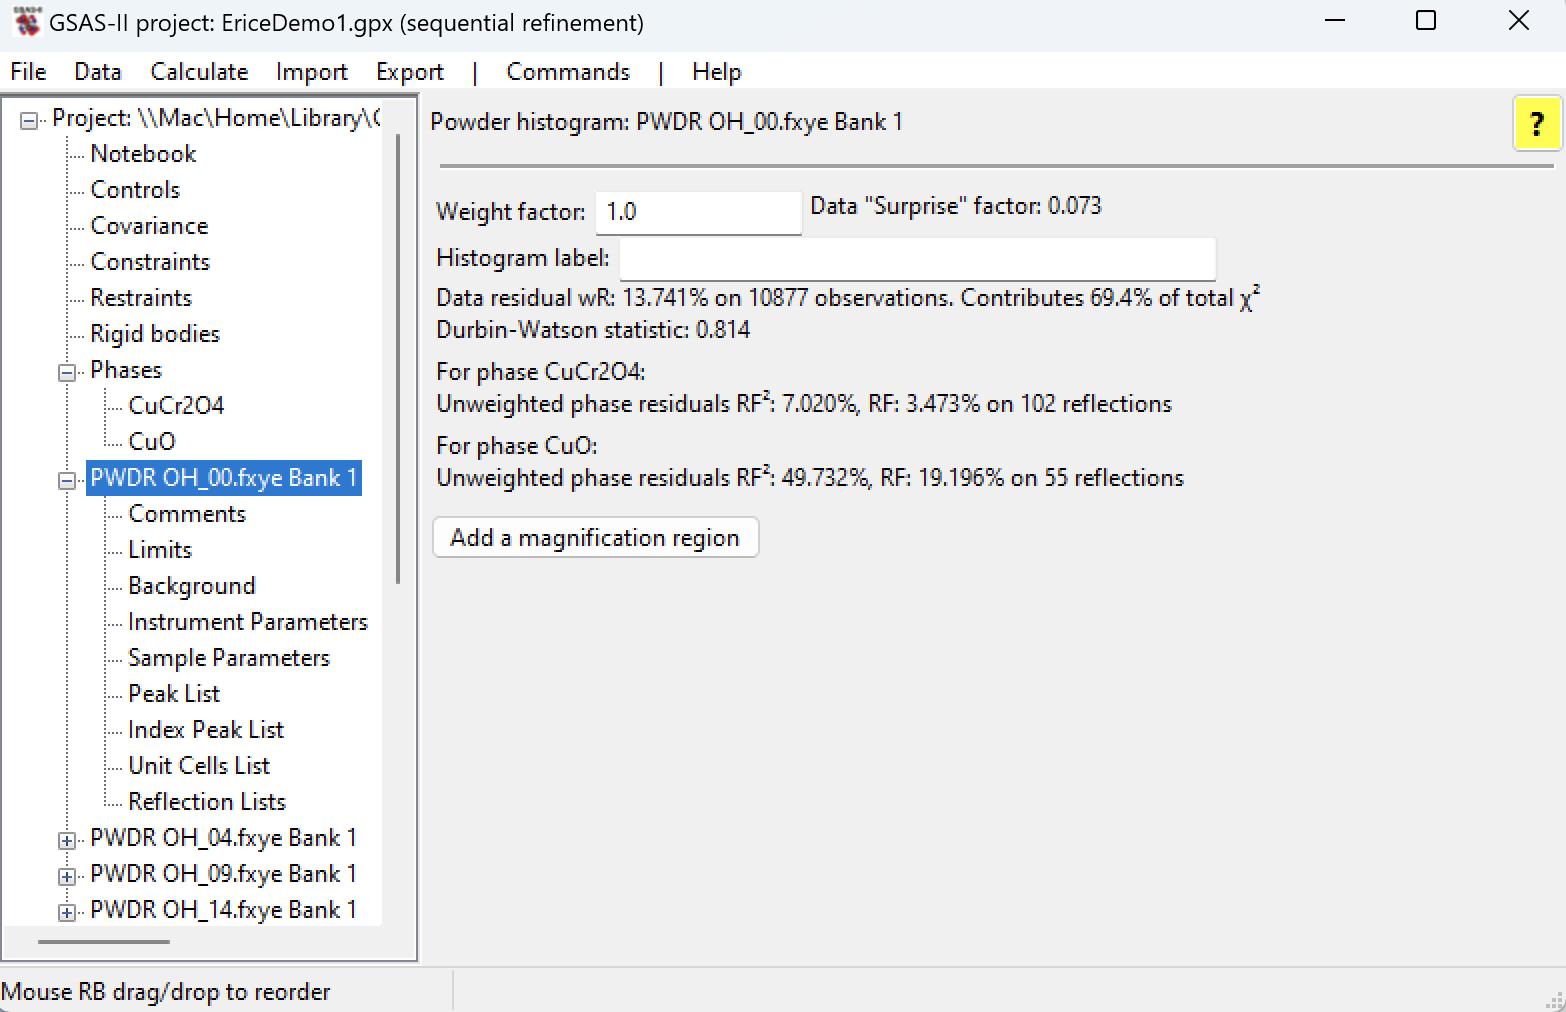
\includegraphics[width=0.5\linewidth]{figures/ScreenMain1.png}
    \caption{An example of the main GSAS-II window where a powder diffraction entry was selected in the left-hand panel where the GSAS-II data tree is located.}
    \label{fig:main1}
\end{figure}
Most input and and interactions with GSAS-II are performed in this window, with the exception of interactions performed with graphics, which will be discussed in the next section. The main window is divided into three sections. For most operating systems, the menu bar is at the top of the window, but on MacOS and a few varieties of Linux, it appears at the top of the screen. On all platforms, the rest of the window is split into two sections. 

The section to the left is the GSAS-II \textbf{data tree}\index{data tree}, where each entry shows a part of the project. In general, the data tree reflects the organization of the data structure that GSAS-II uses to save information on the project. Note that the data tree is hierarchical with two levels of entries, so that the indented entries are subentries of the parent above them. Data tree entries can be overall items found in all projects such as "Notebook" and "Constraints", can contain diffraction data, which will be labeled with a prefix such "PWDR" for powder data or "IMG" for diffraction images. Once a structure (phase) has been imported into a project, a data tree entry named "Phases" will be added to the tree with each phase as a child of that entry. There is no limit in GSAS-II to how many datasets and how many phases may be read into a project. There are other types of entries that can appear in the tree. The "Sequential Results" data tree entry will be discussed later in section \ref{SequentialResults}. 

When an entry or subentry is selected in the data tree, the contents of that selected item is shown to the window section to the right. We call that section the GSAS-II \textbf{data window}.\index{data window}.

Each time a different entry is selected in the data tree, the contents of the data window change and, as well, the contents of the menu change as well, as commands relevant to the selected data tree entry are added. Such commands will appear between two vertical lines (between the "Export" and 
"Help" entries. Note also the yellow question mark button to the upper right. This is the "Help" button and will open a web page that describes the selected data tree item and its associated window. 

In Fig. \ref{fig:main2} a different type of data tree item has been selected, here for a phase. There is enough phase-related information that it cannot be shown in a single window. When that is the case, the GSAS-II GUI will add a set of "notebook tabs", which are found at the top of the data window and will also add a "Select tab" entry to the menu. It is possible to select a tab by clicking on, but when there are too many tabs to fit on the page, rather than using the arrows to scroll the list of tabs, the menu is probably easier to use. Each tab may have a separate help entry.

\begin{figure}
    \centering
    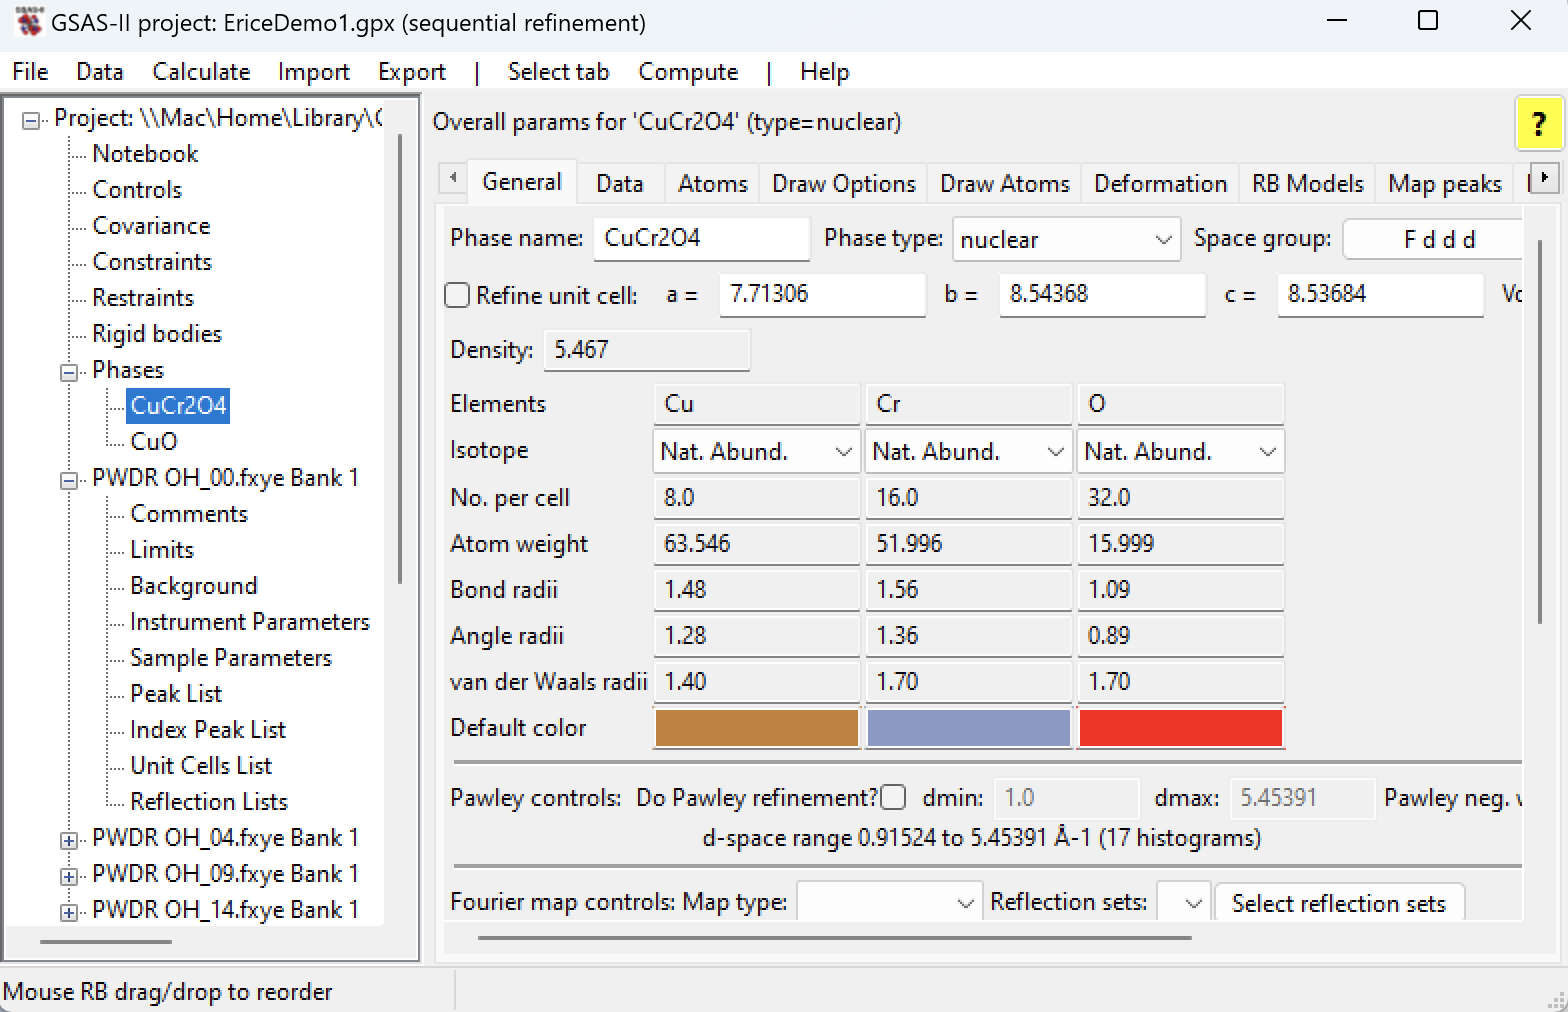
\includegraphics[width=0.5\linewidth]{figures/ScreenMain2.png}
    \caption{An example of the main GSAS-II window where a phase diffraction entry was selected in the data tree in left-hand panel. This selection changes the window contents to the right as well as section of the menu bar between the Export and Help entries (between the two vertical lines).}
    \label{fig:main2}
\end{figure}
\subsection{The GSAS-II graphics window}
A design principle for GSAS-II is to use visualization to help make numerical values more clear and to provide you the ability to provide input graphically wherever appropriate. Many data tree items will cause graphics to be generated. These graphics are placed in a separate window, which is called the GSAS-II graphics window.\index{GSAS-II graphics window} In cases where the data tree window has tabs, there may be a different graphics entry for the tab. The help entry for the data tree entry or tab will document the graphical display as well as the data window contents. The graphics may be 2D or 3D. An example of 2D graphics is shown in Fig. \ref{fig:graphics}. 

As an example of how the graphics window may accept graphical input, consider the example displayed in Fig. \ref{fig:graphics}.  This was generated by clicking on the main data tree entry for a powder diffraction pattern. Note the tickmarks, the small vertical lines near the bottom of the plot that show the reflection positions for each of the two phases that are present. The location of these tickmarks on the plot can be changed by clicking the mouse down on any tickmark and then while holding the mouse down, moving up or down vertically to a new location and releasing the mouse. This is called "dragging" the tickmark. The difference curve (the cyan line showing the observed pattern after subtracting the computed pattern) can be dragged as well.  If instead, the Limits subentry for a powder pattern had been selected, one has access to set the range of data that will be used in the fit and a slightly different plot is shown. The limits can be changed by typing an entry into the appropriate control on the window or by dragging the green or red vertical line.

The toolbar at the bottom of the window provides controls that change the graphics display. It is documented in the GSAS-II help\footnote{URL https://advancedphotonsource.github.io/GSAS-II-tutorials/help/applicationwindow.html\#Plots} 
but a few items are worth a specific mention here. The button labeled "K" shows a menu of keystroke commands. As an example, there is a keystroke command "q". This command will change the plot to display the pattern with the x-axis in Q rather than $2\theta$.  This command can be executed by pressing the "q" keyboard key while the graphics window is active or by selecting the "q" entry in the menu raised when the "K" button is pressed. If you use GSAS-II frequently, you will likely start to remember the keyboard shortcuts for options that you use often, but the "K" button will show you all available options and the help page may provide further explanations. The blue "?" button will open the help page. The green "P" button is used to create version of the current plot that is improved for publication. 

\begin{figure}
    \centering
    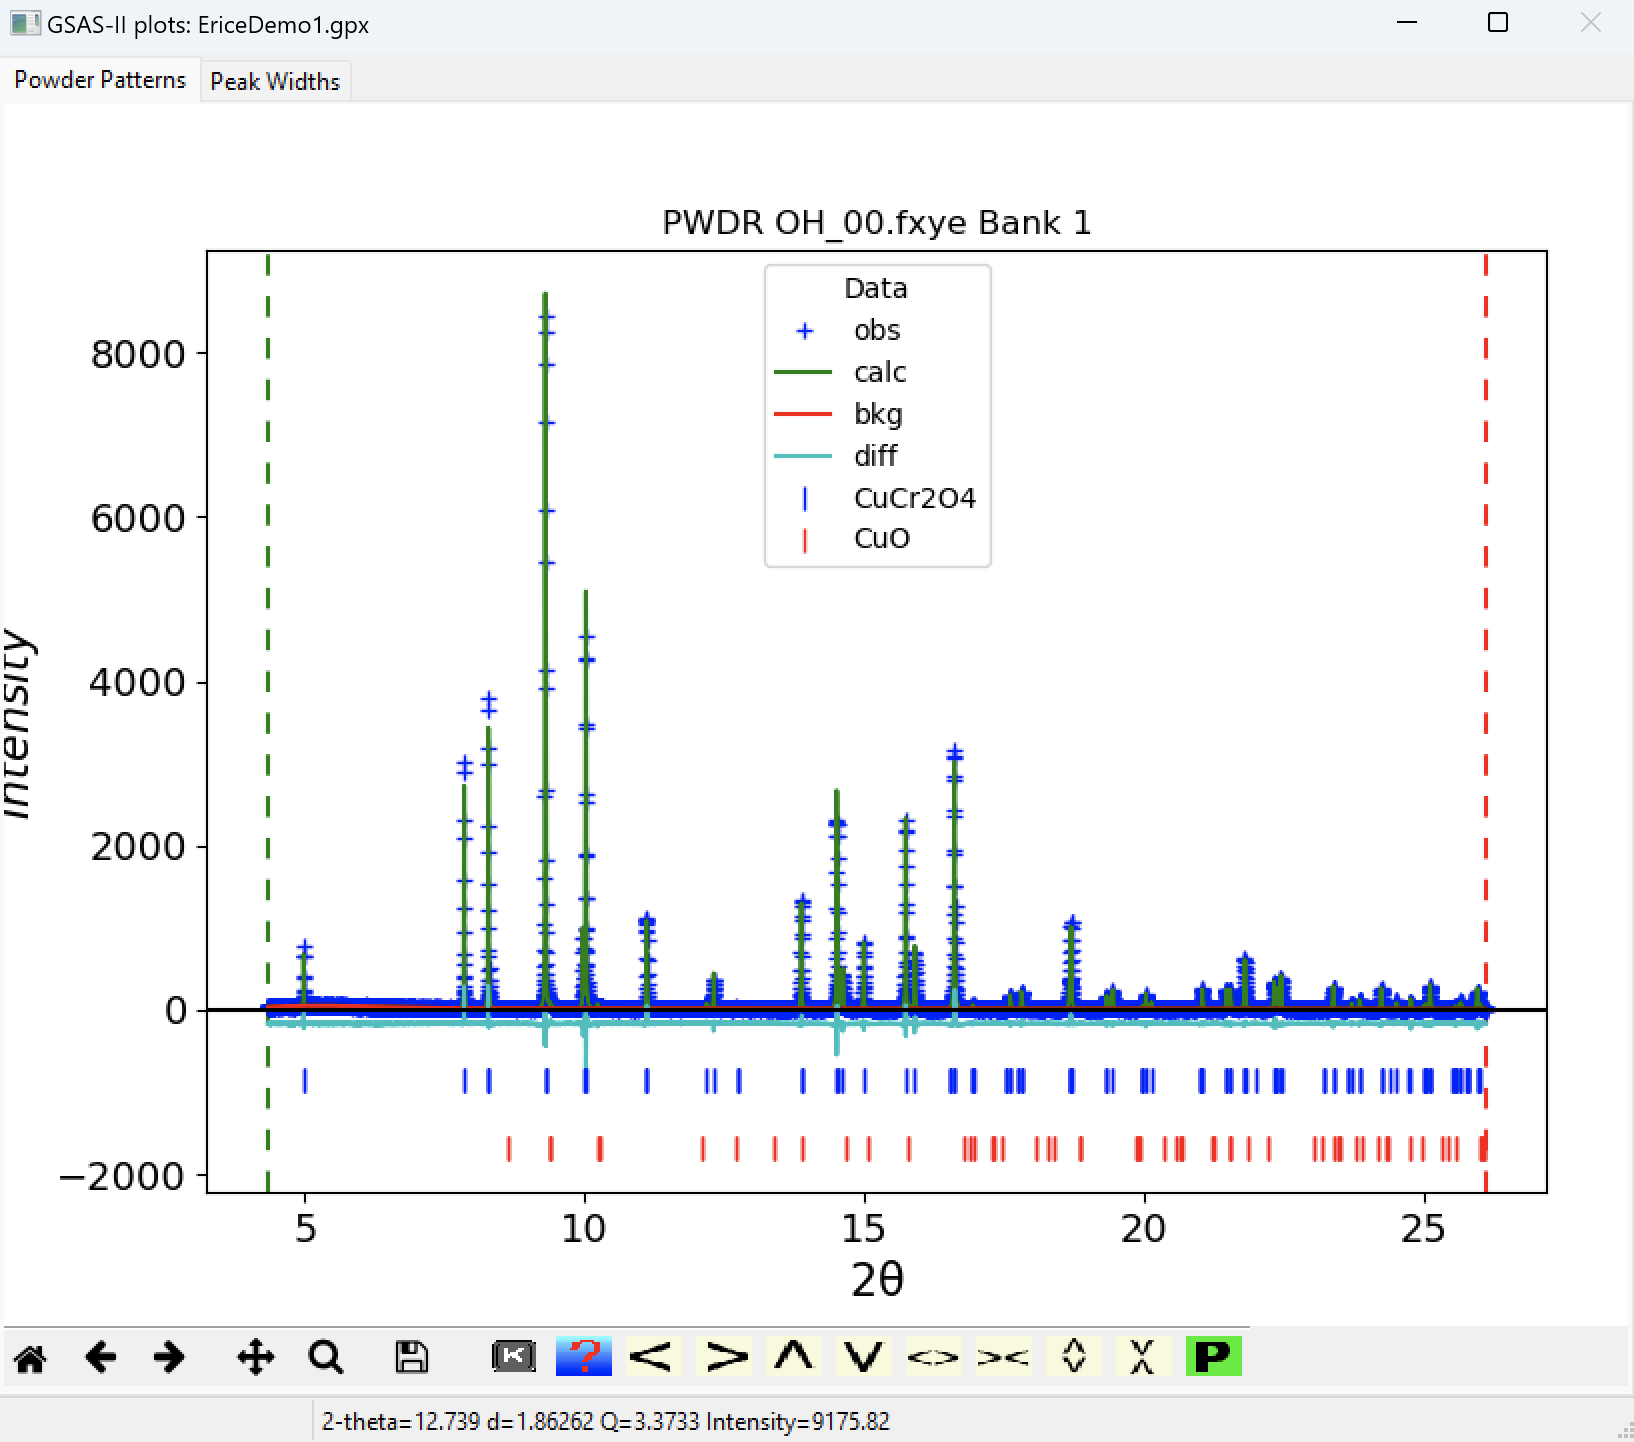
\includegraphics[width=0.5\linewidth]{figures/ScreenGraphics.png}
    \caption{The GSAS-II graphics window. Different plots and visualization information is shown here, depending on actions and selections in the main GSAS-II window. Some graphics are be interactive, responding to mouse actions and keyboard keys.}
    \label{fig:graphics}
\end{figure}
\subsection{The GSAS-II console window}
The final core window opened by GSAS-II is called the GSAS-II console window, as seen in Fig. \ref{fig:console}. It is used for output of status information, such as information on the installed GSAS-II version and the Python and Python package versions that GSAS-II is using. More information is displayed when the "debug" preference option is set to True. The main purpose of this window is to capture information related to problems with GSAS-II. If an error is encountered when running GSAS-II, information about the error will likely appear here. If you are doing something wrong, I hope the console window will help you understand what the problem is. If it is an error in GSAS-II, this information is essential for debugging. We encourage you to report these errors and when you do please include the output in this console window, but also prefer to get a copy of the .gpx file and instructions on how to duplicate the error as well . 

Note that the console window is only used for output from GSAS-II. You will never provide any input to the program in this window. 
\begin{figure}
    \centering
    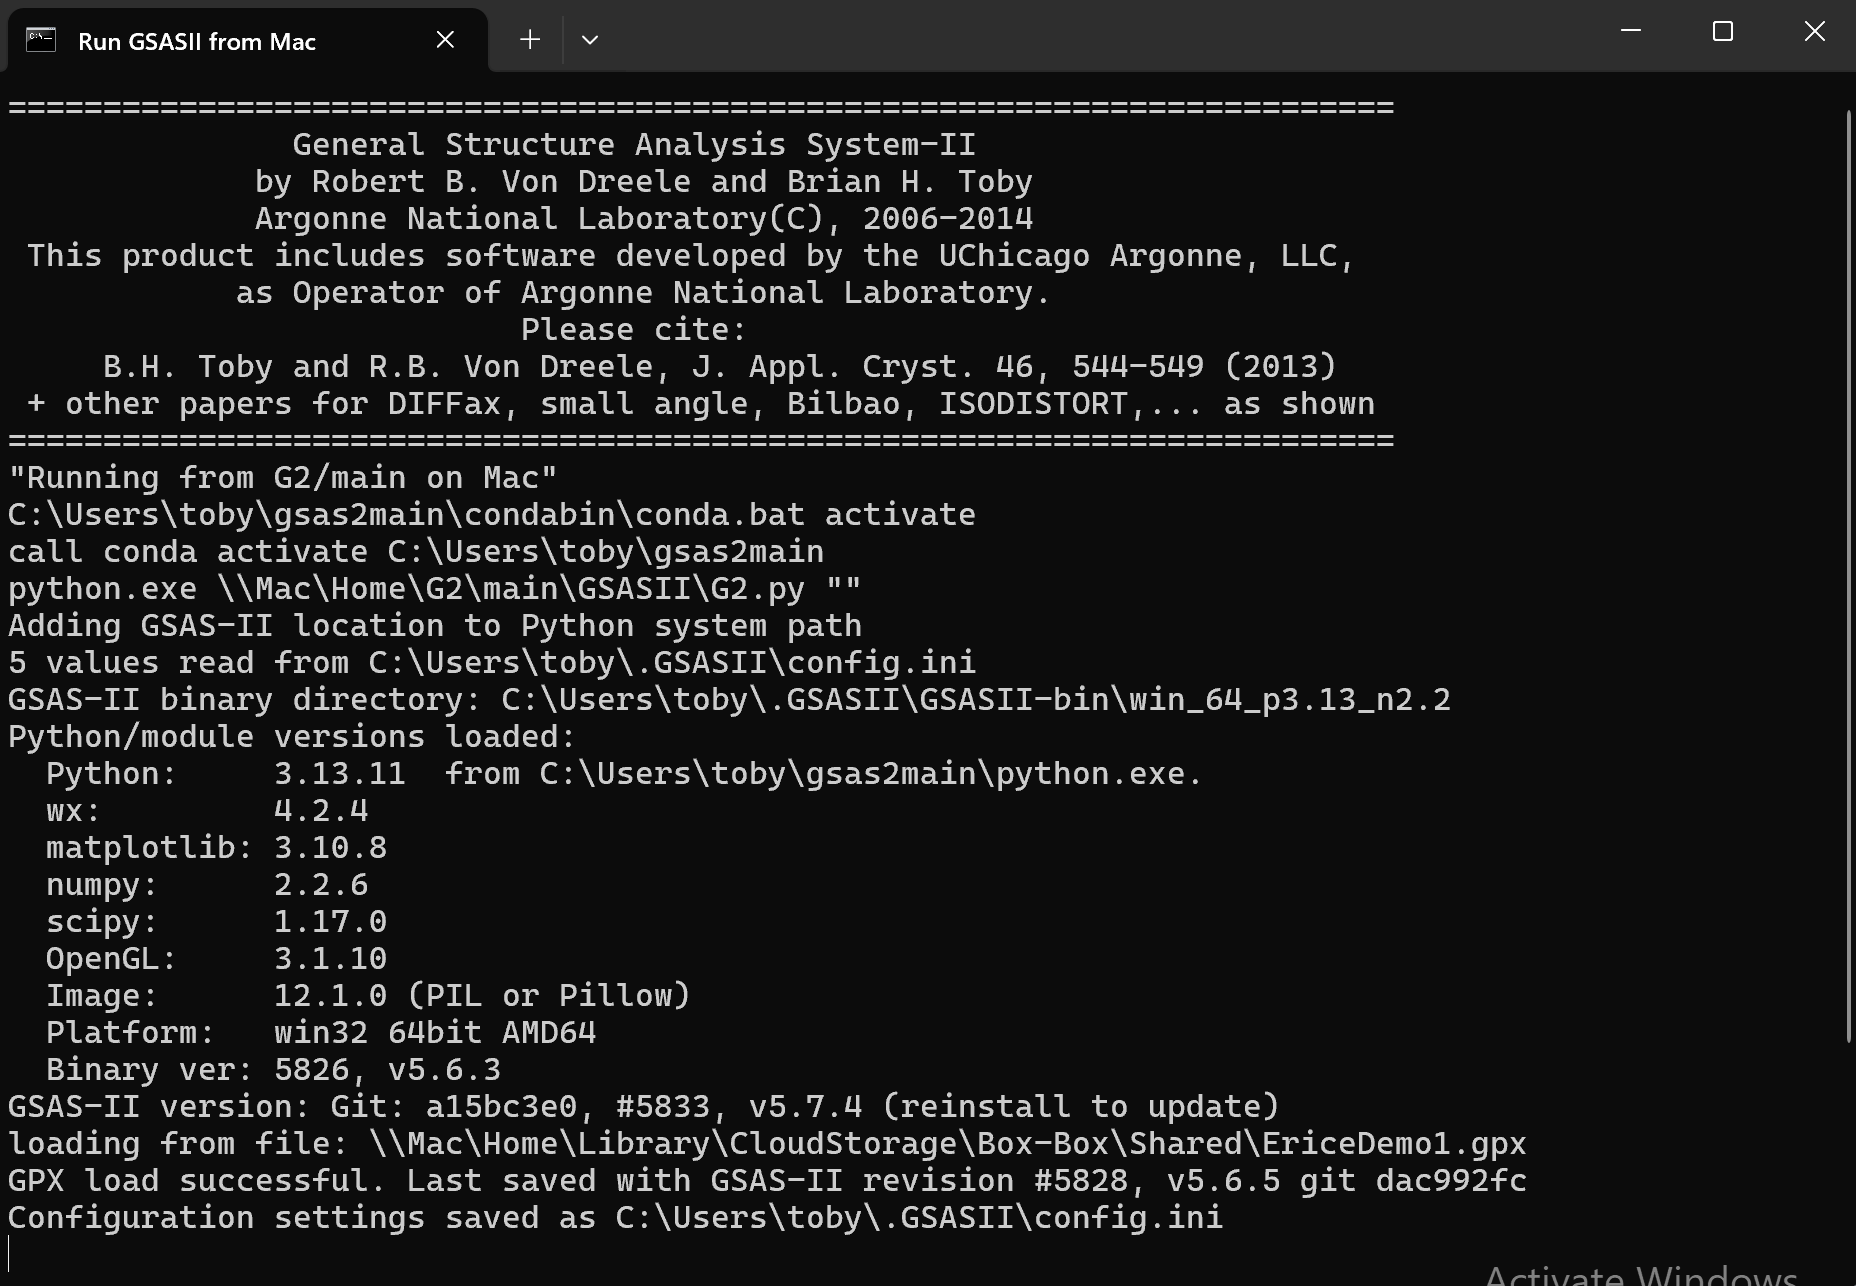
\includegraphics[width=0.5\linewidth]{figures/ScreenConsole.png}
    \caption{The GSAS-II console window. This is used for output only. Status and error messages may appear here. This window is not used for any input.}
    \label{fig:console}
\end{figure}